\documentclass[a4paper,12pt]{article}
\usepackage[margin=1in]{geometry}

\usepackage[T2A]{fontenc}			% кодировка
\usepackage[utf8]{inputenc}			% кодировка исходного текста
\usepackage[english,russian]{babel}	% локализация и переносы
\usepackage{graphicx}                % Математика
\usepackage{amsmath,amsfonts,amssymb,amsthm,mathtools} 
\usepackage{mathtext}
\usepackage[T2A]{fontenc}
\usepackage[utf8]{inputenc}

\usepackage{wasysym}

%Заговолок
\author{Бичина Марина 
группа Б04-005 1 курса ФЭФМ}
\title{}
\date{}


\begin{document} % начало документа

\begin{center}
\begin{Large}
{Корнеев Николай Б04-005, Лабораторная работа №. 4.7.2 <<Эффект Поккельса>>}
\end{Large}
\end{center}
\subsection*{Цель работы:} 
\begin{enumerate}
\itemsep0em
\item Исследовать интерференцию рассеянного света, прошедшего через кристалл
\item Наблюдать изменение характера поляризации света при наложении на кристалл электрического поля
\end{enumerate}
\subsection*{Задание:}
\begin{enumerate}
\itemsep0em
\item Измерив радиусы интерференционных колец, определить разность показателей преломления $n_{o}-n_{e}$
\item Подав на кристалл постоянное напряжение, получить свет, поляризованный по кругу
\item Определить полуволновое напряжение по фигурам Лиссажу на экране осциллографа
\end{enumerate}
\subsection*{Оборудование:}
\begin{enumerate}
\itemsep0em
\item Гелий-неоновый лазер
\item Поляризатор
\item Кристалл ниобата лития
\item Матовая пластинка
\item Экран
\item Источник высоковольтного переменного и постоянного напряжения
\item Фотодиод
\item Осциллограф
\item Линейка
\end{enumerate}


\subsection*{Теоретическая справка:}
\textbf{Эффектом Поккельса} называется изменение показателя преломления света в кристалле под действием электрического поля.

Изменение показателя преломления кристаллов под действием
внешнего электрического поля происходит за счёт анизотропных
свойств кристаллов. Под действием постоянного электрического поля
электроны смещаются в сторону того или иного иона (в случае
кристалла ниобата лития $LiNbO_3$ — это ион Li или Nb), при этом
меняется поляризуемость среды и связанный с ней показатель преломления.

Рассмотрим кристалл ниобата лития $LiNbO_3$ с симметрией вдоль оси $z$. Для световой волны с $\mathbf{E}$ перпендикулярно $z$ показатель преломления будет $n_o$, а для волны с $\mathbf{E}$ вдоль $z$ -- $n_e$. В случае, когда луч света идёт под углом $\theta$ к оси, есть два значение показателя преломления $n_1$ и $n_2$: $n_1 = n_o$ для волны с $\mathbf{E}$ перпендикулярным плоскости $(\mathbf{k},\mathbf{z})$ (обыкновенная волна) и $n_2$ для волны с $\mathbf{E}$ в этой плоскости (необыкновенная волна). В последнем случае
\begin{equation}
\dfrac{1}{n_2^2}=\dfrac{\cos^2 \theta}{n_0^2}+\dfrac{\sin^2 \theta}{n_e^2}.
\end{equation}
Если перед кристаллом, помещённым между скрещенными поляроидами, расположить линзу или матовую пластинку, после которых лучи будут рассеиваться под различными углами, то на экране,
расположенном за поляроидом, мы увидим тёмные концентрические
окружности — результат интерференции

Разность фаз в таком случае равняется:
\begin{equation}
\Delta\varphi=\frac{2\pi}{\lambda}\cdot l\cdot(n_1-n_2)\approx\frac{2\pi}{\lambda}\cdot l\cdot(n_o-n_e)\theta^2
\end{equation}
Тогда выражение для m-го кольца получаем:
\begin{equation}
r^2_{m}=\frac{\lambda}{l}\frac{(n_oL)^2}{n_{o}-n_{e}}m
\label{r}
\end{equation}

Теперь поместим кристалл в постоянное электрическое поле $E_{\text{эл}}$, направленное вдоль оси $x$, перпендикулярной $z$. Показатель преломления для луча, распространяющего вдоль $z$, всегда $n_o$. В плоскости $(x,y)$ возникают два главных направления под углами $45^\circ$ к $x$ и $y$ с показателями преломления $n_0 - \Delta n$ и $n_o + \Delta n$ (быстрая и медленная ось), причём $\Delta n = A\cdot E_{\text{эл}}$. Для поляризованного вертикально света и анализатора, пропускающего горизонтальную поляризацию, на выходе интенсивность на выходе будет иметь вид
\begin{equation}
I_{\text{вых}} = I_0 \sin^2 \left(\dfrac{\pi}{2} \dfrac{U}{U_{\lambda/2}} \right),
\end{equation}
где $U_{\lambda/2} = \frac{\lambda}{4A}\frac{d}{l}$ -- \textit{полуволновое напряжение}, $d$ -- поперечный размер кристалла.  При напряжении $U = E_{\text{эл}}d$ равном полуволновому сдвиг фаз между двумя волнами равен $\pi$, а интенсивность света на выходе максимальна. 

\subsection*{Описание установки:}
\paragraph{Установка для 1 этапа работы}
\begin{figure}[h!]
\centering
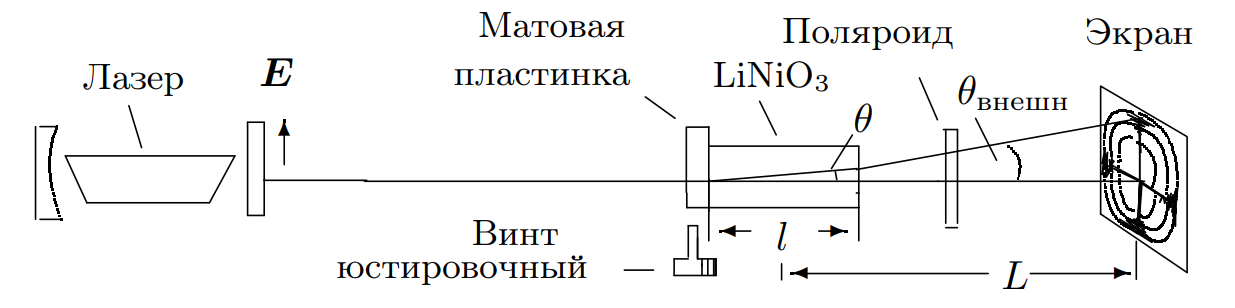
\includegraphics[scale=0.45]{setup.png} 
\caption{Схема установки для наблюдения эффекта Поккельса}
\end{figure}
\begin{enumerate}
\itemsep0em
\item He-Ne лазер, длина волны $\lambda = 0.63$ мкм, $n_o=2.29$
\item Матовая пластинка
\item Кристалл $LiNiO_3$, размером 3х3х26$\;\text{мм}$ 
\item Поляроид
\item Экран
\end{enumerate}
\paragraph{Установка для 2 этапа работы}
\begin{figure}[h!]
\centering
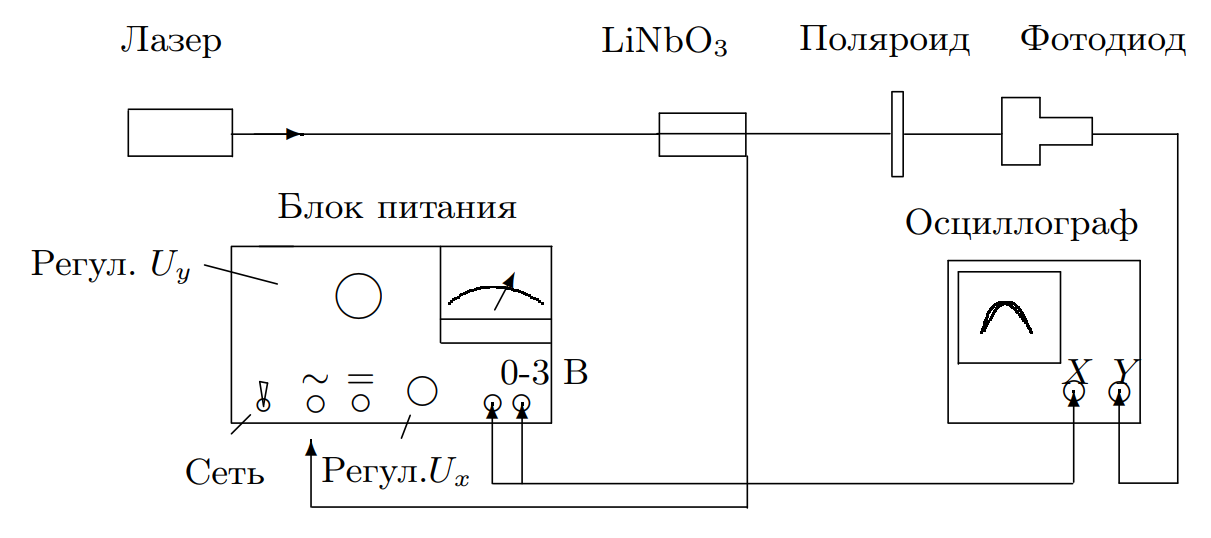
\includegraphics[scale=0.4]{setup_0.png} 
\caption{Схема для изучения двойного лучепреломления в электрическом поле}
\end{figure}
\subsection*{Ход работы:}
\paragraph{Изучение интерференции обыкновенной и необыкновенной волн}
\begin{enumerate}
\itemsep0em
\item Соберем установку, измерим  $L = 87$ см -- расстояние от центра кристалла до экрана.
\item Рассмотрим радиус колец, полученных в ходе интерференции обыкновенной и необыкновенной волн
\begin{table}[h!]
\centering
\begin{tabular}{|l|l|l|l|l|l|l|l|l|l|l|l|}
\hline
№     & 1   & 2   & 3   & 4   & 5   & 6   & 7   & 8   & 9   & 10   & 11   \\ \hline
r, см & 3.4 & 4.6 & 5.6 & 6.5 & 7.3 & 8.0 & 8.6 & 9.2 & 9.8 & 10.4 & 10.8 \\ \hline
\end{tabular}
\end{table} 
\item За погрешность возьмем наибольшую полуширину между кольцами ($\sigma_{r} = 2\;\text{мм}$). Тогда для построения графика мы будем использовать погрешность, равную: $\sigma_{r^2} = 2r\cdot\sigma_{r}\;\text{мм}$ 
\item Построим график $r^2=f(m)$, пользуясь методом наименьших квадратов
\begin{figure}[h!]
\centering
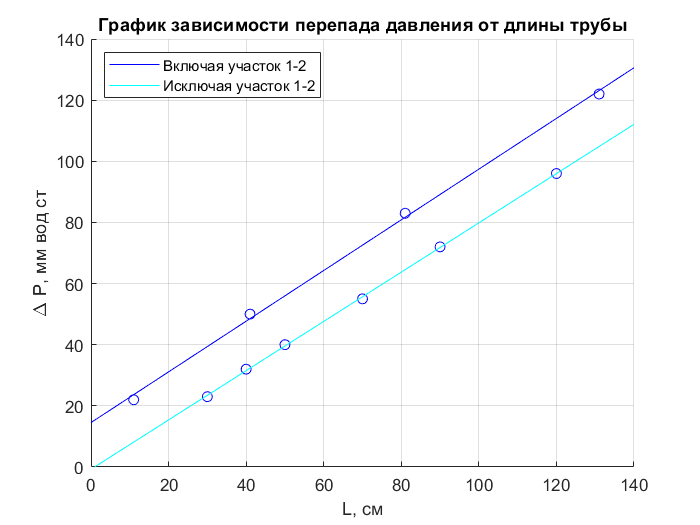
\includegraphics[scale=0.9]{../../../../../Users/Marina/plot_3.pdf} 
\end{figure}
\item Получим угловой коэффициент, равный $k = 10.67\pm 0.07$ см$^2$.
\item По формуле \ref{r} рассчитаем значение разности $(n_{o}-n_{e})$
\begin{equation*}
n_{o}-n_{e} = \frac{\lambda(n_{o}L)^2}{l}\cdot \frac{1}{k} = 0.09
\end{equation*}   
Погрешность в этом случае равна:
\begin{equation*}
\sigma_{n_{o}-n_{e}} = (n_{o}-n_{e})\sqrt{\left( \frac{2\sigma_{L}}{L}\right)^2+\left(\frac{\sigma_{k}}{k}\right)^2} = 0.09\sqrt{\left( \frac{2\cdot 1}{87}\right)^2+\left(\frac{0.07}{10.67}\right)^2}=0.0026\approx 0.003
\end{equation*}
В итоге получим:
\[(n_{o}-n_{e})=0.090\pm 0.003\]
\end{enumerate}
\paragraph{Изучение оптических свойств кристалла под действием электрического поля}
\begin{enumerate}
\itemsep0em
\item Преобразуем установку: уберем матовую пластинку, лист бумаги с экрана. 
\item Будем изменять напряжение: максимум достигается при $U = U_{\lambda/2} = 30\;\text{дел} = 0.45\;\text{кВ}$, минимум при $U = 2U_{\lambda/2} = U_{\lambda}= 56\;\text{дел} = 0.84\;\text{кВ}$
\item Подадим на кристалл напряжение, равное $U = \frac{1}{2}U_{\lambda/2}=U_{\lambda/4}$. При вращении поляризатора яркость пятна не изменяется, значит, поляризация в этом случае круговая. 
\item Вместо экрана поставим фотодиод. В итоге получим установку как на рисунке 2.

 Сменим разъем с постоянного, на переменное напряжение. В этом случае на разъем x будет подаваться напряжение с источника напряжения, а на y - напряжение с фотодиода.  

На экране появится синусоида (фигура Лиссажу). Чем большее напряжение мы подаем, тем больше периодов в фигуре Лиссажу.
\item Далее прикреплены фотографии фигур Лиссажу, полученных в ходе эксперимента. 
\begin{figure}[h!]
\begin{minipage}[h!]{0.4\linewidth}
\centering
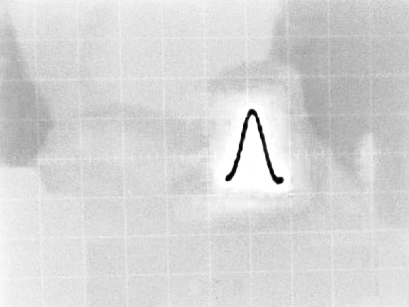
\includegraphics[scale=0.5]{lis_1.png} 
\caption{Фигура Лиссажу при  $U = U_{\lambda/2}$}
\end{minipage}
\hfill
\begin{minipage}[h]{0.4\linewidth}
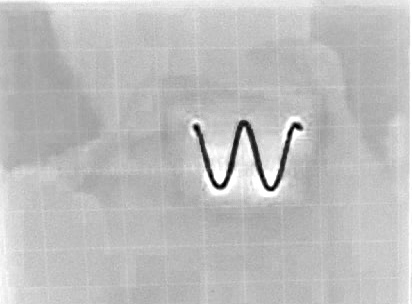
\includegraphics[scale=0.5]{lis_2.png} 
\caption{Фигура Лиссажу при  $U = U_{\lambda}$}
\end{minipage}
\end{figure}
\begin{figure}[h!]
\centering
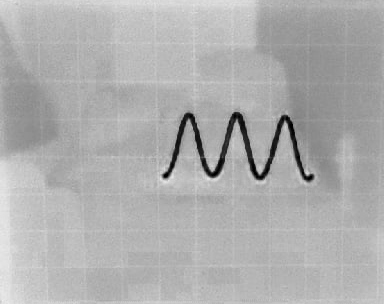
\includegraphics[scale=0.5]{lis_3.png} 
\caption{Фигура Лиссажу при  $U = U_{3\lambda/2}$}
\end{figure}
\item По фигуре Лиссажу определим полуволновое напряжение $U = U_{\lambda/2} = 0.45 \pm 0.02\;\text{кВ}$, где погрешность берется по цене деления источника питания. 
\end{enumerate}
\subsection*{Выводы:}
\begin{enumerate}
\itemsep0em
\item Установили прямую зависимость $r^2(m)$
\item Измерив радиусы интерференционных колец, получили показатель преломления, равный $(n_{o}-n_{e})=0.090\pm 0.003$
\item Подав на кристалл постоянное напряжение, получили свет, имеющий круговую поляризацию
\item Определили полуволновое напряжение на глаз по яркости картины на экране и по фигуре Лиссажу на осциллографе. В итоге, получили одинаковый результат, равный $U = U_{\lambda/2} = 0.45 \pm 0.02\;\text{кВ}$. 
\end{enumerate}
\end{document}